\hypertarget{std__includes_8h}{
\section{include/std\_\-includes.h-\/Dateireferenz}
\label{std__includes_8h}\index{include/std\_\-includes.h@{include/std\_\-includes.h}}
}


included die Header, die standartmäßig benötigt werden  


{\ttfamily \#include $<$time.h$>$}\par
{\ttfamily \#include $<$stdio.h$>$}\par
{\ttfamily \#include $<$iostream$>$}\par
{\ttfamily \#include $<$sstream$>$}\par
{\ttfamily \#include $<$sys/time.h$>$}\par
{\ttfamily \#include $<$fstream$>$}\par
{\ttfamily \#include \char`\"{}ros/ros.h\char`\"{}}\par
{\ttfamily \#include \char`\"{}geometry\_\-msgs/Twist.h\char`\"{}}\par
{\ttfamily \#include \char`\"{}std\_\-msgs/Empty.h\char`\"{}}\par
{\ttfamily \#include \char`\"{}std\_\-msgs/String.h\char`\"{}}\par
{\ttfamily \#include \char`\"{}ar\_\-recog/Tags.h\char`\"{}}\par
{\ttfamily \#include \char`\"{}ar\_\-recog/Tag.h\char`\"{}}\par
{\ttfamily \#include \char`\"{}ardrone\_\-brown/Navdata.h\char`\"{}}\par
{\ttfamily \#include \char`\"{}Math.h\char`\"{}}\par
{\ttfamily \#include \char`\"{}Global.h\char`\"{}}\par
{\ttfamily \#include \char`\"{}Keyboard.h\char`\"{}}\par
Include-\/Abhängigkeitsdiagramm für std\_\-includes.h:\nopagebreak
\begin{figure}[H]
\begin{center}
\leavevmode
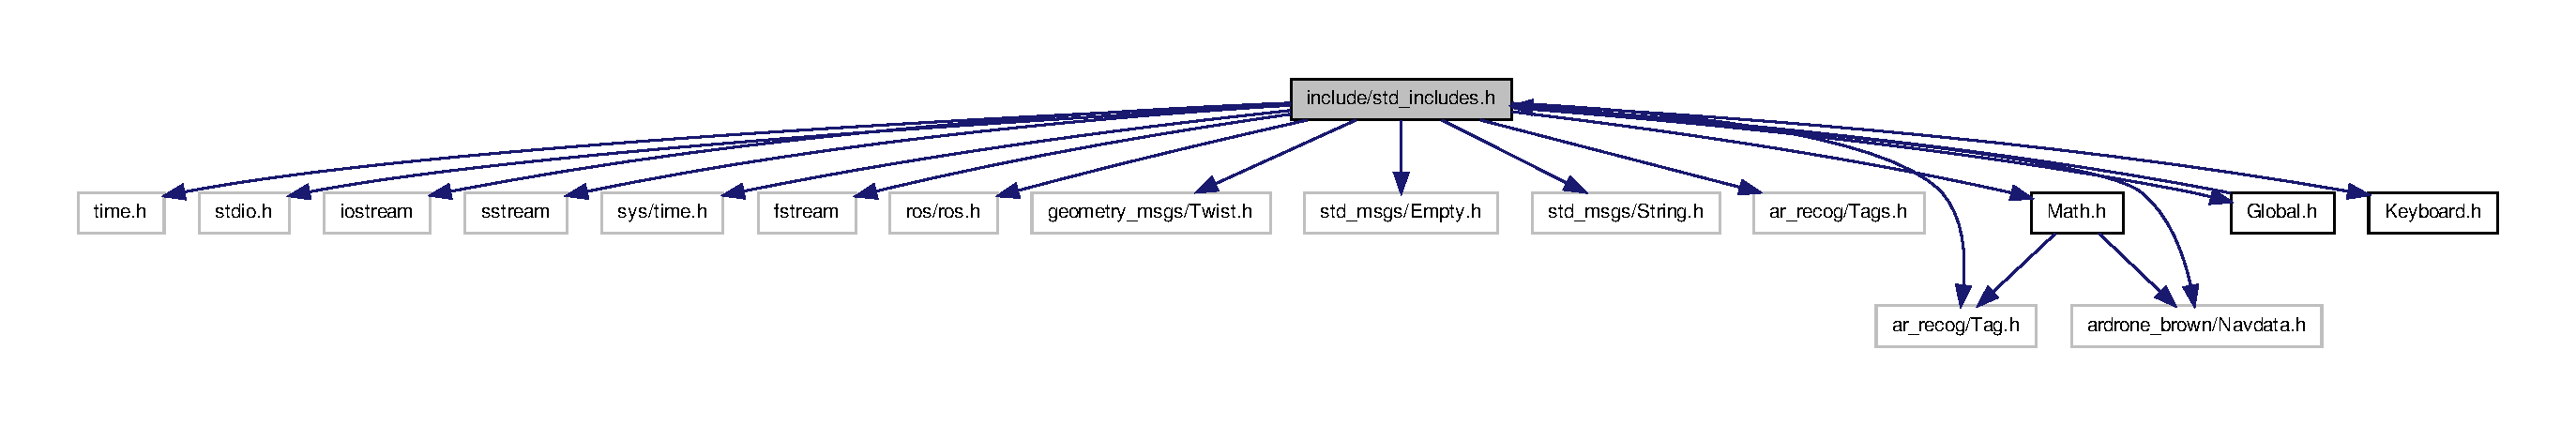
\includegraphics[width=400pt]{std__includes_8h__incl}
\end{center}
\end{figure}
Dieser Graph zeigt, welche Datei direkt oder indirekt diese Datei enthält:\nopagebreak
\begin{figure}[H]
\begin{center}
\leavevmode
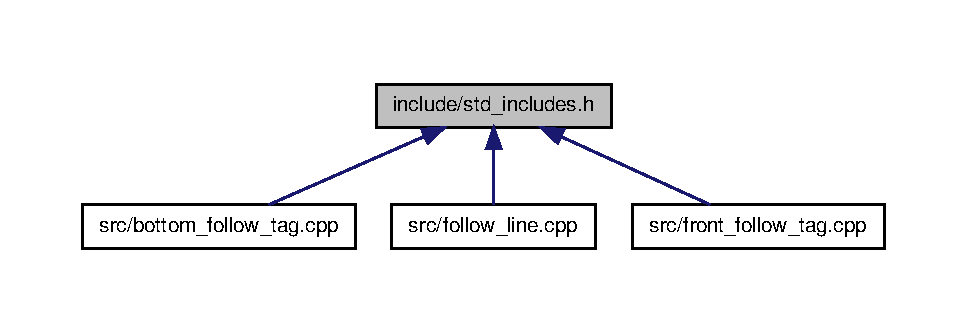
\includegraphics[width=400pt]{std__includes_8h__dep__incl}
\end{center}
\end{figure}


\subsection{Ausführliche Beschreibung}
included die Header, die standartmäßig benötigt werden 

Definiert in Datei \hyperlink{std__includes_8h_source}{std\_\-includes.h}.

